% !TEX program = pdflatex
% Build: latexmk -pdf main.tex
\documentclass[11pt,a4paper]{article}

% ---------- Language and fonts ----------
\usepackage[T1]{fontenc}
\usepackage[utf8]{inputenc}
\usepackage[english]{babel}
\usepackage{lmodern}
\usepackage{microtype}
\usepackage{csquotes}

% ---------- Layout ----------
\usepackage[margin=2.5cm]{geometry}
\usepackage{parskip}

% ---------- Math and units ----------
\usepackage{amsmath}
\usepackage{siunitx}            % \qty{20}{\centi\metre}

% ---------- Figures and tables ----------
\usepackage{graphicx}
\graphicspath{{figures/}}
\usepackage{subcaption}
\usepackage{booktabs}
\usepackage{tabularx}
\usepackage{xcolor}
\usepackage{tikz}
\usetikzlibrary{positioning,arrows.meta,fit}

% ---------- Source code ----------
\usepackage{listings}
\lstset{
  language=Python,
  basicstyle=\ttfamily\small,
  keywordstyle=\color{blue!60!black},
  commentstyle=\color{green!40!black},
  stringstyle=\color{red!60!black},
  numbers=left,
  numberstyle=\tiny\color{gray},
  frame=single,
  rulecolor=\color{gray!50},
  breaklines=true,
  showstringspaces=false,
  captionpos=b
}
\lstdefinelanguage{json}{
  string=[s]{"}{"},
  stringstyle=\color{red!60!black},
  literate={:}{{{\color{gray}:}}}1 {,}{{{\color{gray},}}}1
}

% ---------- References ----------
\usepackage[backend=biber,style=ieee]{biblatex}
\addbibresource{references.bib}

\usepackage[hidelinks]{hyperref}
\usepackage[capitalise,noabbrev]{cleveref}   % must be loaded after hyperref

% ---------- Placeholders ----------
% Search for \todo to find everything that still has to be written.
\newcommand{\todo}[1]{\textcolor{red!75!black}{[TODO: #1]}}

% ---------- Project data ----------
\newcommand{\projecttitle}{Parking Distance Indicator with MQTT and a Web Dashboard}
\newcommand{\coursename}{Practical IoT with Raspberry Pi}
\newcommand{\universityname}{Universidad Politécnica de Madrid}
\newcommand{\schoolname}{Escuela Técnica Superior de Ingeniería y Diseño Industrial}
\newcommand{\departmentname}{Departamento de Electricidad, Electrónica, Automática y Física Aplicada}
\newcommand{\teammembers}{%
  Felix Secherling\\
  Jarno Henrikus Piter van den Ouden\\
  Frieder Bunne}
\newcommand{\submissiondate}{\todo{submission date: 17 December or January, not fixed yet}}
\newcommand{\repourl}{https://github.com/Frieder03/parking-distance-indicator}

\hypersetup{pdftitle={\projecttitle}}

\begin{document}

% ==================== Title page ====================
\begin{titlepage}
  \centering
  \vspace*{3cm}
  {\large \universityname\par}
  \vspace{0.3cm}
  {\schoolname\par}
  \vspace{0.1cm}
  {\departmentname\par}
  \vspace{0.8cm}
  {\large \coursename\par}
  \vspace{2.5cm}
  {\huge\bfseries \projecttitle\par}
  \vspace{0.6cm}
  {\Large Project Report\par}
  \vspace{2.5cm}
  {\large \teammembers\par}
  \vfill
  {\large \submissiondate\par}
\end{titlepage}

\begin{abstract}
  Reversing into a parking space or garage is difficult because obstacles behind
  the car are hard to see. We built a parking distance indicator based on a
  Raspberry Pi. An ultrasonic sensor measures the distance to the nearest
  obstacle. Three LEDs show a green, yellow or red warning, and a buzzer beeps
  faster as the obstacle gets closer. Every measurement is sent over MQTT to a
  web dashboard built with Flask, which shows a car reversing into a parking bay
  in real time. The user can change the warning thresholds and switch the buzzer
  on or off in the browser; the new settings reach the Raspberry Pi over MQTT.
  Tests in simulation confirmed the complete chain from the sensor to the browser
  and back. \todo{one sentence with the main hardware result, e.g.\ measured accuracy}
\end{abstract}

\tableofcontents
\clearpage

% ==================== 1 Introduction ====================
\section{Introduction}
\label{sec:introduction}

\subsection{Motivation}
When a driver reverses, the area directly behind the car is hidden by the car
itself. Low walls, posts, bicycles or children can be missed, and small
collisions during parking are common. Many newer cars have parking sensors, but
older cars and many private garages do not. A simple device that warns the
driver when an obstacle comes too close can prevent this damage.

Our device can be mounted at the back wall of a garage or on the rear of a
vehicle. It warns the driver locally with lights and sound, which works without
any network. In addition, it is connected to the network: the distance can be
watched remotely in a browser, for example by a person guiding the driver, and
the warning thresholds can be adapted to the garage without changing the code.

\subsection{Objectives}
The objective is to build a working prototype of a parking aid. It measures the
distance to the nearest obstacle and warns the user in three levels: green,
yellow and red. As the obstacle gets closer, the warning changes from green to
yellow to red, and the buzzer beeps faster. The measurements are published over
the network and shown on a web dashboard.

We set the following measurable goals:
\begin{itemize}
  \item The sensor measures distances between \qty{5}{\centi\metre} and
        \qty{100}{\centi\metre} with an error below \qty{1}{\centi\metre}.
  \item The LEDs and the buzzer react to a new distance at least four times per
        second.
  \item The dashboard shows a new measurement less than \qty{0.5}{\second} after
        it was taken.
  \item A change of the settings in the browser takes effect on the Raspberry Pi
        within one second.
  \item If the Raspberry Pi stops, the dashboard shows this within a few seconds.
\end{itemize}

\subsection{Scope}
The prototype includes one ultrasonic sensor, three LEDs, a buzzer, the
communication over MQTT and a web dashboard with a REST API. It is built on a
breadboard and tested on a table, not mounted in a real car or garage.

The following points are deliberately left out: several sensors for different
zones behind the car, a weatherproof housing, and a secured network connection
with user accounts and encryption. They are discussed as future work in
\cref{sec:conclusion}.

\subsection{Project Requirements}
\label{sec:requirements}
\Cref{tab:requirements} shows how the prototype meets the course requirements.

\begin{table}[htbp]
  \centering
  \caption{Course requirements and their implementation.}
  \label{tab:requirements}
  \begin{tabularx}{\textwidth}{@{}l X l@{}}
    \toprule
    Requirement & Implementation & Details \\
    \midrule
    Raspberry Pi            & Central controller \todo{model, e.g.\ Raspberry Pi 4 Model B} & \Cref{sec:components} \\
    Sensors                 & Ultrasonic distance sensor & \Cref{sec:components} \\
    Actuators               & Buzzer (acoustic warning) and three LEDs (visual warning) & \Cref{sec:components} \\
    Communication protocols & MQTT between the Raspberry Pi and the dashboard; HTTP with a REST API between the dashboard and the browser & \Cref{sec:communication} \\
    User interface          & Web dashboard with a live parking view and settings & \Cref{sec:webinterface} \\
    Python 3                & All software: measurement, outputs, MQTT client and Flask dashboard & \Cref{sec:software} \\
    \bottomrule
  \end{tabularx}
\end{table}

% ==================== 2 System overview ====================
\section{System Overview}
\label{sec:overview}

\Cref{fig:architecture} shows the structure of the system. The Raspberry Pi
reads the ultrasonic sensor and determines the warning level. It switches the
matching LED and controls the buzzer. After every measurement it publishes the
distance and the warning level to an MQTT broker. The dashboard subscribes to
these messages and serves a web page that shows them. When the user changes a
setting in the browser, the dashboard publishes it over MQTT, and the Raspberry
Pi applies it immediately.

The Raspberry Pi and the dashboard never connect to each other directly; both
only need to reach the broker. The dashboard can therefore run on the Raspberry
Pi itself or on a laptop.

\begin{figure}[htbp]
  \centering
  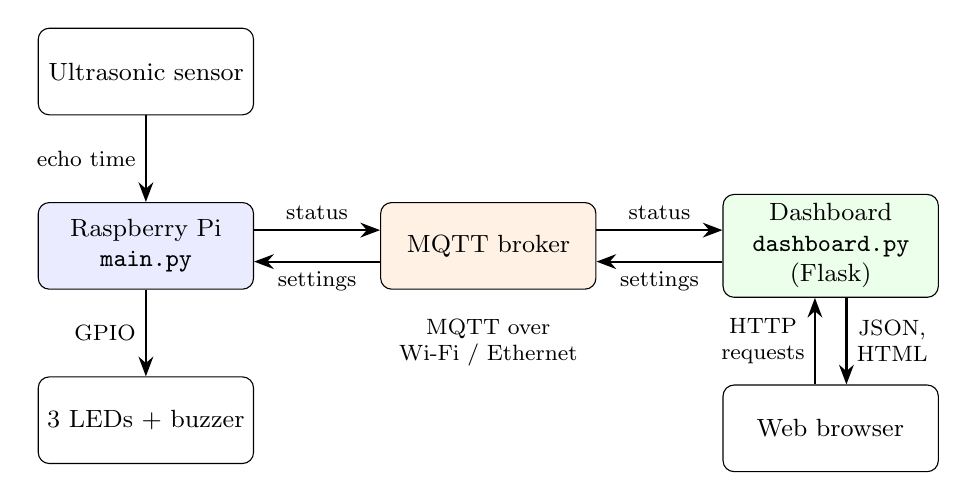
\begin{tikzpicture}[
      font=\small,
      box/.style={draw, rounded corners, align=center, minimum height=1.1cm, text width=2.5cm, fill=#1},
      box/.default=white,
      arrow/.style={-{Stealth[length=2.5mm]}, thick},
      lbl/.style={font=\footnotesize, align=center}
    ]
    \node[box=blue!8]   (pi)     {Raspberry Pi\\\texttt{main.py}};
    \node[box, above=1.1cm of pi]               (sensor) {Ultrasonic sensor};
    \node[box, below=1.1cm of pi]               (out)    {3 LEDs + buzzer};
    \node[box=orange!10, right=1.6cm of pi]     (broker) {MQTT broker};
    \node[box=green!8, right=1.6cm of broker]   (dash)   {Dashboard\\\texttt{dashboard.py}\\(Flask)};
    \node[box, below=1.1cm of dash]             (web)    {Web browser};

    \draw[arrow] (sensor.south) -- node[lbl, left] {echo time} (pi.north);
    \draw[arrow] (pi.south) -- node[lbl, left] {GPIO} (out.north);
    \draw[arrow] ([yshift=2mm]pi.east) -- node[lbl, above] {status} ([yshift=2mm]broker.west);
    \draw[arrow] ([yshift=-2mm]broker.west) -- node[lbl, below] {settings} ([yshift=-2mm]pi.east);
    \draw[arrow] ([yshift=2mm]broker.east) -- node[lbl, above] {status} ([yshift=2mm]dash.west);
    \draw[arrow] ([yshift=-2mm]dash.west) -- node[lbl, below] {settings} ([yshift=-2mm]broker.east);
    \draw[arrow] ([xshift=-2mm]web.north) -- node[lbl, left] {HTTP\\requests} ([xshift=-2mm]dash.south);
    \draw[arrow] ([xshift=2mm]dash.south) -- node[lbl, right] {JSON,\\HTML} ([xshift=2mm]web.north);

    \node[lbl, below=0.25cm of broker] {MQTT over\\Wi-Fi / Ethernet};
  \end{tikzpicture}
  \caption{System architecture. MQTT connects the Raspberry Pi and the dashboard;
           the browser talks to the dashboard over HTTP.}
  \label{fig:architecture}
\end{figure}

% ==================== 3 Hardware ====================
\section{Hardware}
\label{sec:hardware}

\subsection{Components}
\label{sec:components}
\Cref{tab:components} lists the components of the prototype.

\begin{table}[htbp]
  \centering
  \caption{Hardware components.}
  \label{tab:components}
  \begin{tabularx}{\textwidth}{@{}>{\raggedright\arraybackslash}X c l >{\raggedright\arraybackslash}X@{}}
    \toprule
    Component         & Quantity & Type       & Function \\
    \midrule
    Raspberry Pi \todo{model} & 1 & Controller & Reads the sensor, controls the outputs, runs the MQTT client \\
    Ultrasonic sensor HC-SR04 \todo{confirm model} & 1 & Sensor & Measures the distance to the nearest obstacle \\
    LED (green, yellow, red) & 3 & Actuator & Shows the warning level \\
    Buzzer \todo{active or passive, model} & 1 & Actuator & Beeps faster as the distance decreases \\
    Resistor 220 to \qty{330}{\ohm} \todo{exact value} & 3 & Passive & Limits the LED current \\
    Resistors \qty{1}{\kilo\ohm} and \qty{2}{\kilo\ohm} & 1 each & Passive & Voltage divider for the ECHO signal \\
    CanaKit T-cobbler and breadboard & 1 & Wiring & Connects the GPIO header to the breadboard \\
    \bottomrule
  \end{tabularx}
\end{table}

\subsection{Wiring}
\label{sec:wiring}
\Cref{tab:pins} shows the pin assignment. The GPIO numbers follow the BCM
numbering used in the code; the physical pin is the position on the 40-pin
header.

\begin{table}[htbp]
  \centering
  \caption{GPIO pin assignment.}
  \label{tab:pins}
  \begin{tabular}{@{}lrr@{}}
    \toprule
    Part & GPIO (BCM) & Physical pin \\
    \midrule
    Green LED   & 17  & 11 \\
    Yellow LED  & 27  & 13 \\
    Red LED     & 22  & 15 \\
    Sensor TRIG & 23  & 16 \\
    Sensor ECHO (through divider) & 24 & 18 \\
    Buzzer $+$  & 19  & 35 \\
    Buzzer $-$  & GND & 39 \\
    Sensor VCC  & \qty{5}{\volt} & 2 \\
    Sensor GND  & GND & 6 \\
    \bottomrule
  \end{tabular}
\end{table}

\paragraph{Voltage divider.} The HC-SR04 runs on \qty{5}{\volt} and drives its
ECHO pin with \qty{5}{\volt}, but the GPIO inputs of the Raspberry Pi only
tolerate \qty{3.3}{\volt}. A voltage divider with $R_1 = \qty{1}{\kilo\ohm}$ and
$R_2 = \qty{2}{\kilo\ohm}$ reduces the signal:
\begin{equation}
  V_\text{GPIO} = V_\text{ECHO} \cdot \frac{R_2}{R_1 + R_2}
               = \qty{5}{\volt} \cdot \frac{\qty{2}{\kilo\ohm}}{\qty{3}{\kilo\ohm}}
               \approx \qty{3.3}{\volt}.
  \label{eq:divider}
\end{equation}

\paragraph{LED resistors.} Each LED has a series resistor. With a forward voltage
of about \qty{2}{\volt} and a \qty{330}{\ohm} resistor, the current is about
$(\qty{3.3}{\volt} - \qty{2}{\volt}) / \qty{330}{\ohm} \approx \qty{4}{\milli\ampere}$,
well below the limit of a GPIO pin. \todo{adapt to the resistor values used}

\todo{circuit diagram, e.g.\ made with Fritzing}

\subsection{Mechanical Setup}
All components are mounted on one breadboard, which is connected to the
Raspberry Pi with a ribbon cable and a T-cobbler (\cref{fig:prototype}). The
sensor points away from the breadboard towards the obstacle.

\begin{figure}[htbp]
  \centering
  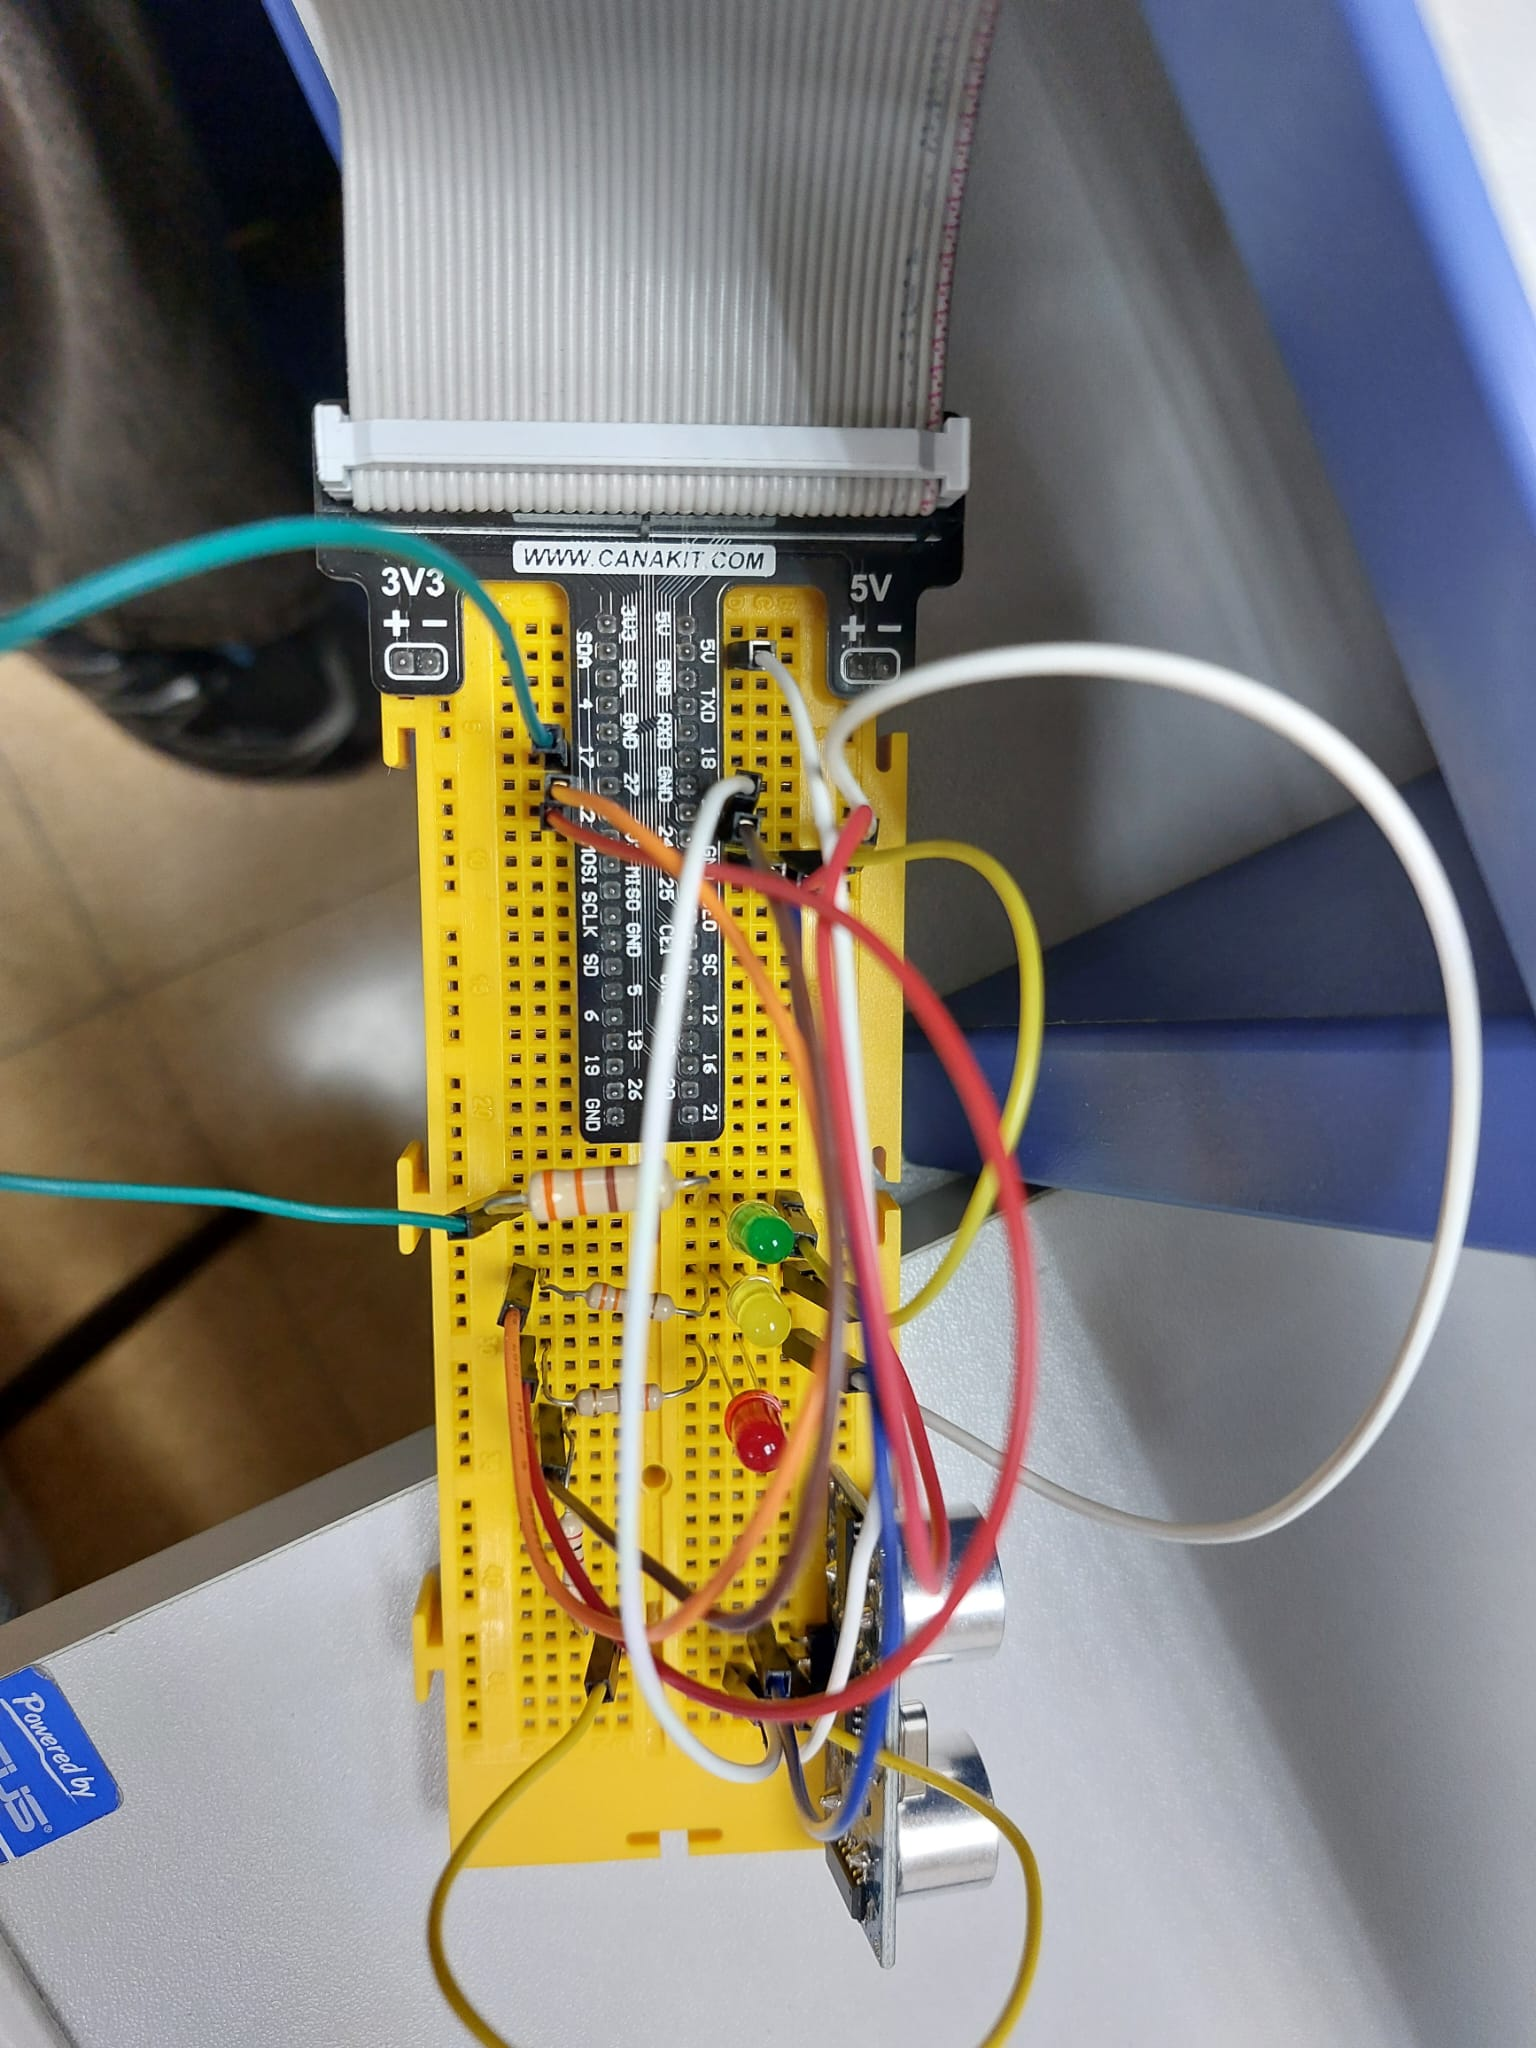
\includegraphics[width=0.45\textwidth]{prototype_breadboard}
  \caption{Prototype on the breadboard with the ultrasonic sensor, the three LEDs
           and the T-cobbler. \todo{replace with a photo of the final setup including the buzzer}}
  \label{fig:prototype}
\end{figure}

% ==================== 4 Software ====================
\section{Software}
\label{sec:software}

\subsection{Program Structure}
All software is written in Python~3. It is split into small modules with one
task each (\cref{tab:modules}). All pins, thresholds, timings and MQTT settings
are collected in \texttt{config.py}, so they can be changed in one place.

\begin{table}[htbp]
  \centering
  \caption{Python modules.}
  \label{tab:modules}
  \begin{tabularx}{\textwidth}{@{}l X@{}}
    \toprule
    Module & Task \\
    \midrule
    \texttt{config.py}    & Pins, thresholds, timing, MQTT broker and topics \\
    \texttt{hardware.py}  & Pin setup and cleanup; selects real or simulated GPIO \\
    \texttt{sensor.py}    & Distance measurement with the ultrasonic sensor \\
    \texttt{leds.py}      & Warning level and LEDs \\
    \texttt{buzzer.py}    & Beep rhythm of the buzzer in a background thread \\
    \texttt{mqtt\_link.py} & MQTT client on the Raspberry Pi: publishes the status, receives settings \\
    \texttt{settings.py}  & Checks and applies settings that arrive over the network \\
    \texttt{main.py}      & Main loop: measure, show the warning, publish \\
    \texttt{dashboard.py} & Flask web server: MQTT subscriber, REST API and web page \\
    \texttt{fake\_gpio.py} & Simulated GPIO and sensor for tests without a Raspberry Pi \\
    \texttt{check\_*.py}  & Small test programs for the LEDs, the sensor and the buzzer \\
    \bottomrule
  \end{tabularx}
\end{table}

The main loop in \texttt{main.py} repeats four steps: it measures the distance,
determines the warning level, updates the LEDs and the buzzer, and publishes the
result over MQTT.

\paragraph{Error handling.} An invalid measurement does not stop the program; it
is reported as \enquote{no valid reading}, all LEDs switch off and the buzzer is
silent. If the MQTT broker cannot be reached, the indicator keeps working
locally, and the MQTT client keeps trying to reconnect in the background.
Settings from the network are checked before they are applied
(\cref{sec:communication}). When the program stops, a \texttt{finally} block
switches off all outputs and releases the GPIO pins.

\paragraph{Simulation mode.} With the option \texttt{--simulate}, the module
\texttt{fake\_gpio.py} replaces the GPIO library. It imitates the sensor with an
obstacle that moves between \qty{4}{\centi\metre} and \qty{60}{\centi\metre}
and sometimes gives no echo. This allowed us to develop and test the warning
logic, the MQTT communication and the dashboard on a laptop.

\subsection{Distance Measurement}
A \qty{10}{\micro\second} pulse on TRIG starts a measurement. The sensor sends an
ultrasonic burst and keeps ECHO high until the echo returns. The distance $d$
follows from this echo time $t$ and the speed of sound $c$:
\begin{equation}
  d = \frac{c \cdot t}{2}, \qquad c \approx \qty{343}{\metre\per\second}
  \text{ at } \qty{20}{\celsius}.
  \label{eq:distance}
\end{equation}
The factor $\frac{1}{2}$ accounts for the way to the obstacle and back.

A single reading is valid if the echo starts and ends within
\qty{50}{\milli\second} and the distance lies between \qty{2}{\centi\metre} and
\qty{400}{\centi\metre}, the range of the sensor. To suppress outliers, each
measurement consists of three readings with a pause of \qty{60}{\milli\second}
in between, so that old echoes fade away. The median of the valid readings is
used. If most readings are invalid, the whole measurement is invalid
(\cref{lst:measurement}). One measurement takes about \qty{0.2}{\second}, which
gives about five updates per second.

\begin{lstlisting}[caption={Median of several readings (\texttt{sensor.py}).},label={lst:measurement}]
def read_distance():
    """Return the median of several pings in cm, or None if most are invalid."""
    readings = []
    for _ in range(config.READINGS_PER_MEASUREMENT):
        distance = read_once()
        if distance is not None:
            readings.append(distance)
        time.sleep(config.PAUSE_BETWEEN_PINGS_S)

    if len(readings) <= config.READINGS_PER_MEASUREMENT // 2:
        return None
    return statistics.median(readings)
\end{lstlisting}

\subsection{Warning Logic}
\label{sec:warning}
The distance determines the warning level. With the default thresholds, the level
is red below \qty{10}{\centi\metre}, yellow below \qty{30}{\centi\metre} and
green otherwise. Only the LED of the current level is on. Without a valid
reading, all LEDs are off. Both thresholds can be changed from the dashboard.

The buzzer behaves as follows:
\begin{itemize}
  \item It is silent in the green zone and when there is no valid reading.
  \item In the yellow zone it beeps for \qty{80}{\milli\second}, and the time
        between two beeps decreases with the distance.
  \item In the red zone it sounds continuously.
\end{itemize}
In the yellow zone, the time $T$ between the beginnings of two beeps changes
linearly with the distance $d$:
\begin{equation}
  T(d) = T_\text{min} + \frac{d - d_\text{red}}{d_\text{yellow} - d_\text{red}}
         \left(T_\text{max} - T_\text{min}\right),
  \label{eq:beep}
\end{equation}
with $T_\text{min} = \qty{0.15}{\second}$ just above the red threshold
$d_\text{red}$ and $T_\text{max} = \qty{0.8}{\second}$ at the yellow threshold
$d_\text{yellow}$.

The buzzer runs in its own thread. The main loop only passes the latest
distance; the thread produces the beeps. This keeps the rhythm steady while the
main loop waits for echoes. When the obstacle comes closer during a pause, the
pause ends early, so the rhythm reacts at once. The code supports an active
buzzer, which is switched on and off directly, and a passive buzzer, which
receives a \qty{2}{\kilo\hertz} PWM signal.

\subsection{Communication}
\label{sec:communication}
The project uses two protocols: MQTT between the Raspberry Pi and the dashboard,
and HTTP with a REST API between the dashboard and the browser.

\paragraph{Why MQTT.} MQTT~\cite{mqtt311} is a lightweight publish/subscribe
protocol designed for IoT devices. Clients do not talk to each other directly;
they publish messages to a topic on a broker, and the broker forwards them to all
clients that subscribed to this topic. For our project this has three
advantages: the Raspberry Pi does not need to know who is watching, the
dashboard can run on any computer that reaches the broker, and further
subscribers, such as a data logger, can be added without changing the code on
the Raspberry Pi. We use the Python client Eclipse Paho~\cite{paho}. The broker
is the public test broker \texttt{test.mosquitto.org}; it can be replaced by our
own Mosquitto broker~\cite{mosquitto} on the Raspberry Pi with one setting.

\paragraph{Topics.} All topics start with
\texttt{etsidi/iot/friederbunne/parking} (\cref{tab:topics}).

\begin{table}[htbp]
  \centering
  \caption{MQTT topics.}
  \label{tab:topics}
  \begin{tabularx}{\textwidth}{@{}l l c c X@{}}
    \toprule
    Topic & Direction & QoS & Retained & Content \\
    \midrule
    \texttt{.../status}   & Pi $\to$ dashboard & 0 & no  & Distance, level and active settings (JSON), after every measurement \\
    \texttt{.../settings} & dashboard $\to$ Pi & 1 & yes & Thresholds and buzzer on/off (JSON) \\
    \texttt{.../online}   & Pi $\to$ dashboard & 1 & yes & \texttt{1} while the Pi runs, \texttt{0} when it stops \\
    \bottomrule
  \end{tabularx}
\end{table}

A status message looks as follows:
\begin{lstlisting}[language=json,numbers=none,caption={Example of a status message.},label={lst:status}]
{"time": 1764165770.2, "distance_cm": 23.4, "level": "yellow",
 "red_below_cm": 10, "yellow_below_cm": 30, "buzzer": true}
\end{lstlisting}

The choice of the MQTT options follows the importance of the messages:
\begin{itemize}
  \item \textbf{QoS 0 for the status.} A new status follows about
        \qty{0.2}{\second} later, so a lost message does not matter, and QoS~0
        causes the least traffic.
  \item \textbf{QoS 1 and retained for the settings.} A change of the settings
        must arrive. Because the message is retained, the broker stores it and
        delivers it to the Raspberry Pi again after a restart.
  \item \textbf{Last will for the online status.} When the Raspberry Pi
        connects, it registers the message \texttt{0} as its last will. If the
        connection is lost, for example because the power is cut, the broker
        publishes this message, and the dashboard shows that the device is
        offline.
\end{itemize}

\paragraph{Checking the settings.} Anyone who can reach the public broker could
publish to the settings topic. Therefore both the dashboard and the Raspberry Pi
check every settings message: it must be valid JSON, contain exactly the three
known fields, and the thresholds must satisfy
$\qty{2}{\centi\metre} \le d_\text{red} < d_\text{yellow} \le \qty{400}{\centi\metre}$.
Invalid messages are ignored.

\paragraph{REST API.} A browser cannot speak MQTT directly, so the dashboard
offers a REST interface~\cite{fielding2000rest} over HTTP (\cref{tab:rest}).
Resources are addressed by URLs, the HTTP method states the action, and the data
is exchanged as JSON.

\begin{table}[htbp]
  \centering
  \caption{REST API of the dashboard.}
  \label{tab:rest}
  \begin{tabularx}{\textwidth}{@{}l l X@{}}
    \toprule
    Method & URL & Function \\
    \midrule
    \texttt{GET} & \texttt{/}              & Web page of the dashboard \\
    \texttt{GET} & \texttt{/api/status}    & Latest distance and level, whether the Pi is online \\
    \texttt{GET} & \texttt{/api/settings}  & Active thresholds and buzzer state \\
    \texttt{PUT} & \texttt{/api/settings}  & Changes the settings; answers \texttt{202} if accepted, \texttt{400} with a reason if invalid, \texttt{503} without a broker connection \\
    \bottomrule
  \end{tabularx}
\end{table}

\subsection{Web Interface}
\label{sec:webinterface}
The dashboard is built with the Flask web framework~\cite{flask}. It shows a
parking bay seen from above (\cref{fig:dashboard}). The car moves towards the
wall as the measured distance decreases, and the red and yellow zones are drawn
according to the current thresholds. The page also shows:
\begin{itemize}
  \item the distance in centimetres and the warning level in its colour,
  \item whether the Raspberry Pi and the MQTT broker are connected,
  \item sound waves at the sensor that follow the beep rhythm while the buzzer
        is on, and brake lights that light up in the red zone,
  \item a form to change both thresholds and to switch the buzzer on or off.
\end{itemize}
The page requests \texttt{/api/status} every \qty{250}{\milli\second} and updates
itself without reloading. If no status message has arrived for
\qty{3}{\second}, the dashboard marks the Raspberry Pi as offline.

\begin{figure}[htbp]
  \centering
  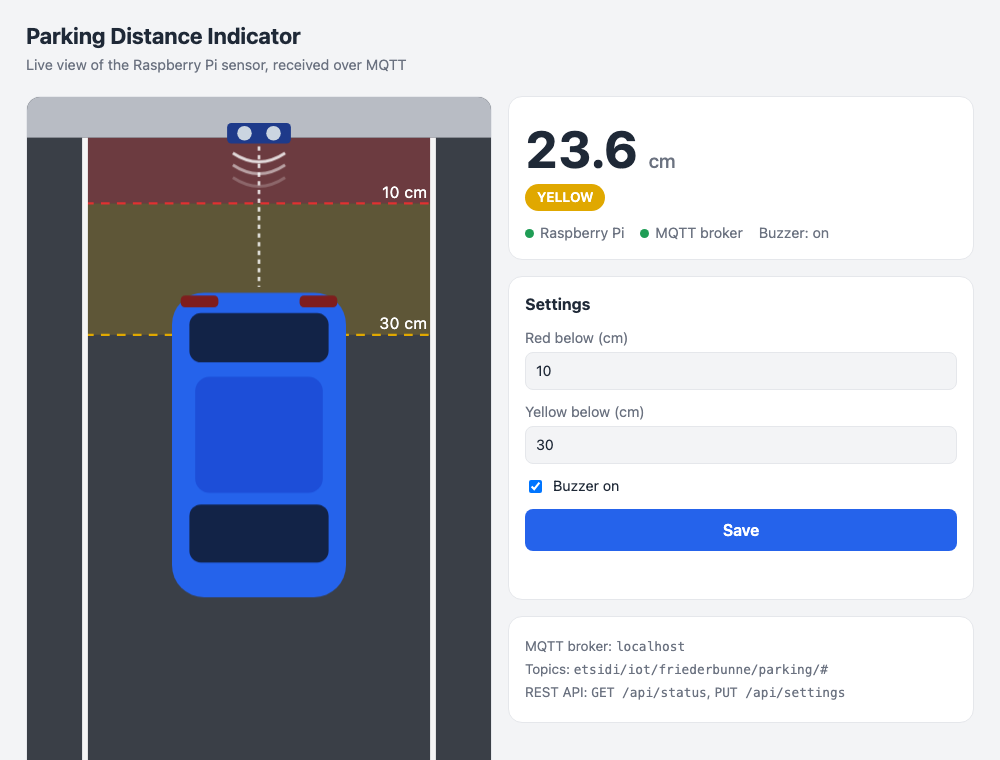
\includegraphics[width=\textwidth]{dashboard}
  \caption{Web dashboard during a test in simulation mode. The obstacle is in the
           yellow zone at \qty{23.6}{\centi\metre}, and the buzzer is beeping.
           \todo{replace with a screenshot from the real prototype}}
  \label{fig:dashboard}
\end{figure}

% ==================== 5 Tests and results ====================
\section{Tests and Results}
\label{sec:results}

The prototype was tested in three steps: the software in simulation, each
component on the Raspberry Pi, and finally the complete system.

\subsection{Software Tests in Simulation}
Before the hardware was complete, the software was tested on a laptop in
simulation mode with a local Mosquitto broker. The following points were
verified:
\begin{itemize}
  \item \textbf{Status chain.} The simulated measurements arrived at the
        dashboard over MQTT, and \texttt{/api/status} returned the current
        distance and level.
  \item \textbf{Settings chain.} A \texttt{PUT} request with
        $d_\text{red} = \qty{15}{\centi\metre}$ and the buzzer switched off was
        answered with \texttt{202}. The Raspberry Pi program applied the new
        settings, and the following status messages contained them.
  \item \textbf{Validation.} A \texttt{PUT} request with
        $d_\text{red} = \qty{40}{\centi\metre}$, which is above the yellow
        threshold, was rejected with \texttt{400} and an explanation.
  \item \textbf{Offline detection.} After the Raspberry Pi program was stopped,
        the dashboard reported the device as offline.
  \item \textbf{Beep rhythm.} At \qty{20}{\centi\metre}, \cref{eq:beep} gives
        $T = \qty{0.475}{\second}$. The recorded switching times of the buzzer
        pin showed beeps every \qty{0.48}{\second}.
\end{itemize}

\subsection{Component Tests}
Each part was first tested on its own with a small program:
\texttt{check\_leds.py} switches on each LED for one second,
\texttt{check\_sensor.py} prints single distance readings, and
\texttt{check\_buzzer.py} plays beeps that get faster, followed by a continuous
tone. Problems found in these tests are described in \cref{sec:discussion}.

\todo{confirm that all three checks pass on the final setup}

\subsection{Sensor Accuracy}
The readings of the sensor are compared with a tape measure at several distances
(\cref{tab:accuracy}). An obstacle with a flat, hard surface, such as a book, is
placed in front of the sensor, and the median of ten measurements is noted.

\todo{carry out the measurement and fill in the table}

\begin{table}[htbp]
  \centering
  \caption{Measured distance compared with the reference distance.}
  \label{tab:accuracy}
  \begin{tabular}{@{}ccc@{}}
    \toprule
    Reference (\unit{\centi\metre}) & Measured (\unit{\centi\metre}) & Error (\unit{\centi\metre}) \\
    \midrule
    5   & --- & --- \\
    10  & --- & --- \\
    20  & --- & --- \\
    30  & --- & --- \\
    50  & --- & --- \\
    100 & --- & --- \\
    \bottomrule
  \end{tabular}
\end{table}

\subsection{System Test}
Finally, the complete system runs on the Raspberry Pi with the dashboard open in
a browser. This test verifies that the LEDs, the buzzer and the dashboard follow
an obstacle that moves towards the sensor, that a threshold changed in the
browser changes the warning on the prototype, and that the dashboard shows the
device as offline when the Raspberry Pi is disconnected.

\todo{results, including the delay between a movement and the update on the dashboard}

\subsection{Planned Demonstration}
We will slowly move an obstacle towards the sensor. The LEDs change from green
to yellow to red, the buzzer beeps faster and finally continuously, and the car
on the dashboard drives towards the wall. We will then leave the obstacle in
place and change the red threshold in the browser to show that the warning on
the prototype changes immediately. Finally, we will unplug the network or stop
the program on the Raspberry Pi to show that the dashboard detects the lost
device through the MQTT last will.

% ==================== 6 Discussion ====================
\section{Discussion}
\label{sec:discussion}

\paragraph{Problems and solutions.} Several problems occurred during the
development:
\begin{itemize}
  \item \textbf{Red LED.} In an early test the red LED did not light up because
        it was missing on the breadboard. Testing each LED on its own with
        \texttt{check\_leds.py} made the error easy to find.
  \item \textbf{Buzzer always on.} The buzzer sounded as soon as it was
        connected, even before the program was started. Setting the pin by hand
        with \texttt{pinctrl} showed that the GPIO pin had no influence on the
        buzzer: it was plugged into a breadboard row that carried a supply
        voltage. We moved the buzzer to a free area and connected it to GPIO~19.
  \item \textbf{5\,V on the ECHO pin.} The sensor outputs \qty{5}{\volt}, which
        could damage the Raspberry Pi. The voltage divider in
        \cref{eq:divider} solves this.
  \item \textbf{Library version.} The package manager of Raspberry Pi OS installs
        version~1.6 of the Paho MQTT client, but our code uses the interface of
        version~2. We therefore install the libraries in a virtual environment,
        and the program states the reason if an old version is found.
  \item \textbf{Network.} Some networks block the public broker. In this case we
        run our own Mosquitto broker on the Raspberry Pi. For the
        demonstration, the Raspberry Pi and the laptop use the same mobile
        hotspot, which avoids restrictions of the university network.
\end{itemize}

\paragraph{Limitations.}
\begin{itemize}
  \item One sensor only covers a narrow cone directly in front of it. Obstacles
        at the side, thin posts and soft surfaces that absorb sound may not be
        detected.
  \item The speed of sound depends on the air temperature. The code assumes
        \qty{20}{\celsius}; at \qty{0}{\celsius} the distance would be about
        \qty{3.5}{\percent} too large.
  \item The public broker is unencrypted and has no user accounts. Anyone could
        read the measurements or send settings. The validation limits the
        possible damage, but a real product would need TLS and authentication.
  \item The dashboard polls the server every \qty{250}{\milli\second}. Pushing
        new data to the browser, for example with WebSockets, would be faster
        and cause less traffic.
\end{itemize}

\todo{interpretation of the accuracy and system test results}

% ==================== 7 Conclusion ====================
\section{Conclusion and Future Work}
\label{sec:conclusion}
We built a parking distance indicator that warns the user with three LEDs and a
buzzer and sends every measurement over MQTT to a web dashboard. The dashboard
shows a live view of the parking situation and lets the user change the
thresholds and the buzzer from any browser. The prototype meets all course
requirements: it runs on a Raspberry Pi, uses a sensor and actuators,
communicates over MQTT and HTTP, offers a web user interface and is programmed
in Python~3.

\todo{state which goals from the objectives were reached, based on the results}

Possible extensions are:
\begin{itemize}
  \item \textbf{Several sensors.} Two more sensors at the left and right rear
        corners would cover the full width of the car. The dashboard could show
        each zone separately.
  \item \textbf{Temperature compensation.} A temperature sensor such as the
        Si7021 could correct the speed of sound,
        $c \approx (331.3 + 0.606\,\vartheta/\unit{\celsius})\,\unit{\metre\per\second}$.
  \item \textbf{Security.} A broker with TLS and user accounts would protect the
        data and the settings.
  \item \textbf{Data logging.} A further MQTT subscriber could store all
        measurements, for example to count parking manoeuvres.
\end{itemize}

% ==================== References ====================
\printbibliography[heading=bibintoc]

% ==================== Appendix ====================
\appendix
\section{Source Code}
\label{app:code}
The complete source code and the installation instructions are available at
\url{\repourl}.

To run the prototype on the Raspberry Pi:
\begin{lstlisting}[language=bash,numbers=none]
git clone https://github.com/Frieder03/parking-distance-indicator.git
cd parking-distance-indicator/code
python3 -m venv --system-site-packages .venv
source .venv/bin/activate
pip install "paho-mqtt>=2" flask
python3 main.py          # terminal 1: sensor, LEDs, buzzer, MQTT
python3 dashboard.py     # terminal 2: web dashboard on port 5001
\end{lstlisting}

\end{document}
